\chapter{Introduction}

Advances in manufacturing and hardware design have made mobile robots more accessible for not only research and industrial purposes, but to the general public. However, autonomous robots have largely been limited to indoor, carefully controlled environments. Before autonomous robots can be more widely deployed, they must be able to accurately observe and represent unstructured, dynamic environments. Dense sensors such as light field cameras are becoming cheaper and lighter, promising to allow autonomous robots to acquire detailed measurements of complex environments. To fully utilise the potential of these advancing technologies, improvements in observer design are required to generate more accurate and detailed descriptions of these environments from dense measurements.

One method of estimating the state of a complex environment is with an \textit{infinite-dimensional observer}. Typically, observers for infinite-dimensional systems are extensions of finite-dimensional Luenberger observers. Unfortunately, this design approach is only able to guarantee convergence for linear systems. Developing a theory of symmetry-preserving, infinite-dimensional observers would simplify the design process for nonlinear systems and result in observers with improved convergence properties.

This research project serves as an initial exploration into the design of symmetry-preserving, infinite-dimensional observers. An infinite dimensional system will be simplified and an observer will be designed to estimate a finite dimensional state. The potential for a symmetry-preserving, infinite-dimensional observer to improve performance will be explored. 

This report presents the novel implementation of an observer to estimate the state of a rigid cube from range measurements. Section \ref{sec:literature} reviews the current state of observer design methods for infinite-dimensional systems. Recent work in the development of design methodologies for symmetry preserving observers is described. Particular attention is paid to a dense optical flow estimator that will be particularly relevant to this research.
 
Chapter \ref{chap:background} provides theory on Lie groups, rigid body state representation and state observer concepts that will be relevant in the observer design.

The cube state estimation problem that is the focus of this research is described in detail in Chapter \ref{chap:problem}. The place of this problem within the larger area of symmetry-preserving, infinite-dimensional observer research is defined.  

Chapter \ref{chap:simulation} provides a detailed description of the simulation implementation, including the observer update function design. The performance of the observer in estimating the state of stationary and moving cubes is assessed. It is shown that almost global convergence is achieved for orientation and size correction for stationary cubes, though the position update only converges in special cases.

Chapter \ref{chap:experiment} details steps taken to experimentally validate the results of the simulation. Range measurement data is collected and used to develop an error distribution model for the Hokuyo UBG-04LX-F01 sensor. Range measurements of a cube of known trajectory are taken for future performance testing.

\section{Literature review} \label{sec:literature}
The use of dense sensors allows for a more accurate estimation of the state of an infinite-dimensional system such as a complex, real-world environment. The theory of infinite-dimensional observers is required to fully utilise this information. This section will review the current state of design methodologies and implementations for infinite-dimensional observers. Particular focus will be paid to an emerging avenue of research; symmetry-preserving observer design. Recent theory developments in this area have allowed limitations in the global convergence properties of nonlinear observers to be overcome.

\subsection{Infinite-dimensional observers}
In many real world systems the dependent variables are functions of one or more spatial variables. An example would be the dynamics of waves in a body of water. The height of the surface varies continuously along the $x$ and $y$ directions. These spatial variables vary continuously, meaning an infinite number of parameters is required to describe the state of the system. Such systems are termed \textit{infinite-dimensional systems}, or \textit{distributed parameter systems}. Their dynamics are modelled by a partial differential equation (PDE). 

When a state estimate is required but direct measurement of the state with sensors is difficult or impossible, a \textit{state observer} is employed. A state observer is a filter that provides an estimate of the state of a system using the difference between its measured and predicted outputs. A more detailed description of the concept of a state observer is provided in Section \ref{sec:observerequations}. An observer for an infinite-dimensional system is called an \textit{infinite-dimensional observer}.

\subsubsection{Linear systems}
Observer theory for \textit{linear} infinite-dimensional systems has been widely studied. The techniques used are typically extensions of Luenberger observers and Kalman filter methods used to observe finite dimensional system.

A simplified approach is to use a spatial discretisation method such as finite difference or finite element to reduce the infinite-dimensional system to a finite-dimensional one. From here, finite-dimensional observer design techniques can be used. This is known as the \textit{early lumping} method, and was employed by Stavroulakis \cite{stavroulakis1973design} who implemented a finite-dimensional observer as part of a control system for an infinite dimensional systems.

The early lumping approach suffers from \textit{spillover}, a phenomenon where performance is affected by the neglected dynamics of the system\cite{meirovitch1983problem}. Harkort \cite{harkort2011finite} recently developed an observer based control scheme that reduced this effect by using modelled outputs rather than true measurements to reduce the effect of the neglected dynamics.

More accurate observers can be designed with the \textit{late lumping} approach which uses the infinite-dimensional model of the system in the observer design. The result is an infinite-dimensional observer that is discretised later for practical implementation. These methods are typically extensions of Kalman or Luenberger methods to infinite dimensions. 

Early work by Gressang \cite{gressang1975observers} extended the Luenberger observer to infinite-dimensional systems whose state space was an abstract Banach space with dynamics defined by an infinitesimal generator of a semigroup. More recently, Smyshlyaev \cite{smyshlyaev2005backstepping} developed an exponentially converging backstepping observer for systems governed by parabolic PDEs. Ramdani introduced forward and backward observers \cite{ramdani2010recovering} whose convergence properties were investigated by Haine \cite{haine2014recovering}.

\subsubsection{Nonlinear systems}
There is currently no universal approach for observer design for nonlinear infinite-dimensional systems.
The most common approach has been to linearise the system, then apply a linear infinite-dimensional observer design. Common linearisation methods include Lyapunov methods, extended linearisation and the Lie-algebraic approach \cite{primbs1996survey}.

There has been some progress in infinite-dimensional observer design for special cases of nonlinear systems. For bilinear systems, Xu \cite{xu1995observer} designed an infinite-dimensional observer that converged for certain inputs. Bounit \cite{bounit1997observers} designed Kalman and Luenberger type observers for infinite-dimensional bilinear systems. 

Despite these small advances in special cases of nonlinear design, the most common design methods for nonlinear infinite-dimensional systems are based on linearisation techniques. These techniques rely on the fact that differentiable functions can be approximated by a first-order Taylor expansion around a point. Luenberger and Kalman methods can be applied to linear approximations of infinite-dimensional systems around an equilibrium point. This simplification relies on the dynamics of system at the point of linearisation being representative of the entire space. In general, this is not necessarily true, and is the biggest limitation in this design technique. The result is that these linearised observers only converge if the initial state estimate is within a local neighbourhood of the true state. Global converge is not guaranteed which severely limits robustness.

Global convergence can be achieved by taking account the symmetries inherent to the system during observer design. A powerful tool for dealing with symmetries is the theory of \textit{Lie groups}. Investigation into \textit{symmetry-preserving} observer design for systems on Lie groups is an active area of research. It promises to produce theoretically validated design principles for nonlinear infinite-dimensional observers, though the majority of research so far has been limited to finite-dimensional observers.

\subsection{Symmetry-preserving observers}
The motivation behind symmetry-preserving observers is to take advantage of invariances in the dynamics of the system. The goal is to design an observer around an equilibrium point in such a way that it can be extended to converge around a wider set of points.

\subsubsection{Early work}
Geometry conscious observer design is not a new idea. Early investigation by Marcus \cite{marcus1984algebraic} into algebraic and geometric methods for nonlinear filter design showed promise.
A seminal work by Salcudean \cite{salcudean1991globally} was the design of an eventually-exponential, globally converging observer for the attitude of rigid bodies from orientation and torque measurements. This observer design took advantage of the simplicity of the quaternion rotation representation and dynamics of rigid body motion.

Another important result that is a precursor to the active research of today is a design method developed by Aghannon \& Rouchon \cite{aghannan2002invariant}. Their invariant observer construction was based on Cartan's moving frame method. Though convergence was proven for a specific problem, the observer convergence for a general case was left an open problem. Maithripala \cite{maithripala2005intrinsic} demonstrated the effectiveness of Aghannon \& Rouchons' method by incorporating it into the design of an intrinsic observer based controller. Performance was shown to be independent of the coordinate system used to represent the configuration space.

\subsubsection{Active research}
There are currently two groups actively researching symmetry-preserving observer design.  Both have begun to apply symmetry-preserving methods to infinite-dimensional observers.

The work of Bonnabel, Auroux, Rouchon, Martin et al. is a progression of the early results from Aghannon \& Rouchon. Their general approach is to first design a Luenberger type observer around an equilibrium point. An invariant frame is used to construct an invariant output error. The observer innovation term respects the symmetries of the system and thus the nonlinear observer is well behaved around a continuum of equilibrium points. 

In \cite{bonnabel2005invariant}, Bonnabel et a. developed an observer design procedure based on Aghannon \& Rouchons' work. Asymptotic stability was achieved, though this required a design procedure tailored to specific nonlinearities of the system and did not apply in a general case.
It was shown in \cite{bonnabel2008symmetry} that an invariant error equation simplified convergence analysis. The observer's global behaviour improved, having a larger region of attraction in comparison to naively linearised observers.
Developments were made to the theory and presented in \cite{bonnabel2009non}. For a particular class of invariant system it was shown that the observer converged locally around any trajectory, and global convergence behaviour was independent of trajectory.

Most recently, these invariant design methods were applied to an infinite dimensional system \cite{auroux2011symmetry}. An observer estimating the state of fluid in a water tank where height varied with the continuous dependent variables position and time was developed. It was shown to converge more quickly and robustly than previous attempts to design infinite dimensional observers with Extended Kalman Filter (EKF) methods.

The work of Trumpf, Mahony, Hamel, Lageman et al. differs in scope. The methods of Bonnabel et al. are generalised and can be applied to a wide range of systems. In contrast, the work of Trumpf et al. is limited to two specific classes of systems but achieves stronger convergence properties.
In \cite{mahony2009nonlinear} nonlinear filters on the Special Orthogonal Group $\mathbf{SO}(3)$ are used in attitude estimation and the resulting nonlinear observers achieved almost globally stable observer error.
Another attitude observer \cite{trumpf2012analysis} achieved almost globally asymptotic and locally exponential convergence.
In \cite{mahony2013observers}, the design methodology for 2 classes of systems is presented. The approach taken is to lift the kinematic system onto its symmetry group and design an observer for the lifted system. The Lyapunov method is used to design the observer innovation term. This methodology simplifies nonlinear observer design and produces observers with strong convergence properties. This group has also begun research  on symmetry-preserving infinite-dimensional observers.

The motivation behind the development of infinite-dimensional observers is to allow dense sensors to be fully utilised. In this vein, research presented in a PhD thesis by Zarrouati \cite{zarrouati2013augmented} utilised dense measurements from a camera and depth sensor. An observer was developed from rotation invariant equations for light and depth. Though the sensors took measurements of an infinite dimensional state, a finite dimensional approximation of this state is what was estimated by the observer.

Another recent work by Adarve et al.\cite{adarvefiltering} also uses dense sensing in the estimation of an infinite dimensional state. This result will be examined closely as it is similar in direction to this research.

Adarve et al. design an update-propagation filter to iteratively compute dense optical flow $\Phi$ from CCD camera measurements $Y$. In reality, this optical flow is an infinite dimensional state. Rather than computing the optical flow independently at each frame, a two-stage process is used to build it incrementally. The propagation stage uses a non-linear PDE to model the transport of the optical flow in the next time step. The update stage corrects this prediction using the current image.

The iterative filter used in this approach is an observer that estimates the state of the continuous spatio-temporal flow field. By using a dense sensor, the measured image stream can be treated as a continuous, infinite-dimensional state. This is in contrast to sparse optical flow computation where the image is modelled as a set of discrete pixel values. However, the flow field $\Phi$ is discretised and computed in $r$ independent regions $\Omega$ around a discrete set of control points $\xi$ as shown in Figure \ref{fig:flow}. Here, this approach differs from that of general infinite-dimensional invariant observer. The state is treated as a discrete set of locally continuous states which does not allow for symmetry considerations. This is because the PDE relations in the local regions are invariant to 2D rotation and translation, but the interactions between regions themselves are not. 

\begin{figure}
\centering
  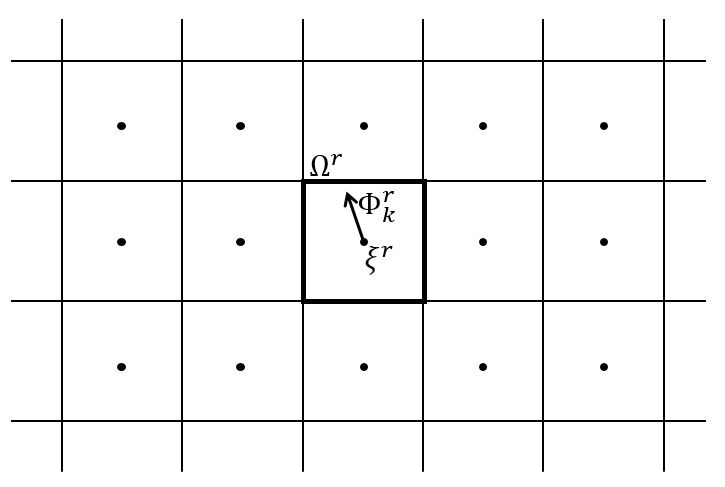
\includegraphics[width=0.8\textwidth,trim = 0mm 0mm 0mm 0mm,clip]{./Figures/flow_regions.jpg}
  \caption{Infinite dimensional optical flow discretised and computed in separate, independent regions} \label{fig:flow_regions}
\end{figure} \label{fig:flow}

Discretising $\Phi$ and $Y$ at the beginning of the algorithm design makes this is an example of the early lumping design approach. Employing a late lumping approach by discretising an infinite dimensional observer would allow for the rotation and translation invariance of the flow field to be taken advantage of to improve convergence properties. 

The lesson to take from this analysis is that discretisation methods must be carefully chosen in order to preserve the invariance of the observer.

Another reason to pay attention to geometric symmetries in observer design is due to limitations placed on convergence by the topology of the system. Bhat \& Bernstein \cite{bhat2000topological} show that global convergence cannot be achieved with a continuous observer on a state space that includes a vector bundle such as $\mathbf{SE}(3)$. Some advancements have been made with extended state-space observers \cite{huang2000analysis,talole2010extended}, that extend the state space. However, this scheme can produce state estimates that are incompatible with the physics of the system prior to convergence. A theory of symmetry-preserving observer design for infinite dimensional systems could simplify observer design and convergence analysis for such systems.


